\documentclass[xetex,table,aspectratio=169]{beamer}

\usepackage[autostyle]{csquotes}
\usepackage{hyperref}
\usepackage{color}
\usepackage{xcolor}
\usepackage{setspace}
\usepackage{listings}
\usepackage{minted}
\usepackage{booktabs}
\usepackage{fancyvrb}
\usepackage{fontawesome}

\usetheme{metropolis}

\setbeamertemplate{section in toc}[circle]

\usemintedstyle{perldoc}
\definecolor{codebackground}{rgb}{0.96,0.96,0.75}

\newcommand{\myhref}[2]{
  \href{#1}{#2 {\tiny\faExternalLink{}}}
}

\title{Supporting Video (de)serializers in Linux:\\Challenges and Works in Progress}
\author{Luca Ceresoli --- AIM Sportline\\
  \href{mailto:luca@lucaceresoli.net}{\tt luca@lucaceresoli.net}\\
  \url{http://lucaceresoli.net}
}
\date{\href{https://events19.linuxfoundation.org/events/embedded-linux-conference-europe-2019/}{Embedded Linux Conference Europe 2019}}

\begin{document}

\maketitle

\begin{frame}{About me}
  \begin{columns}
    \column{0.5\textwidth}
    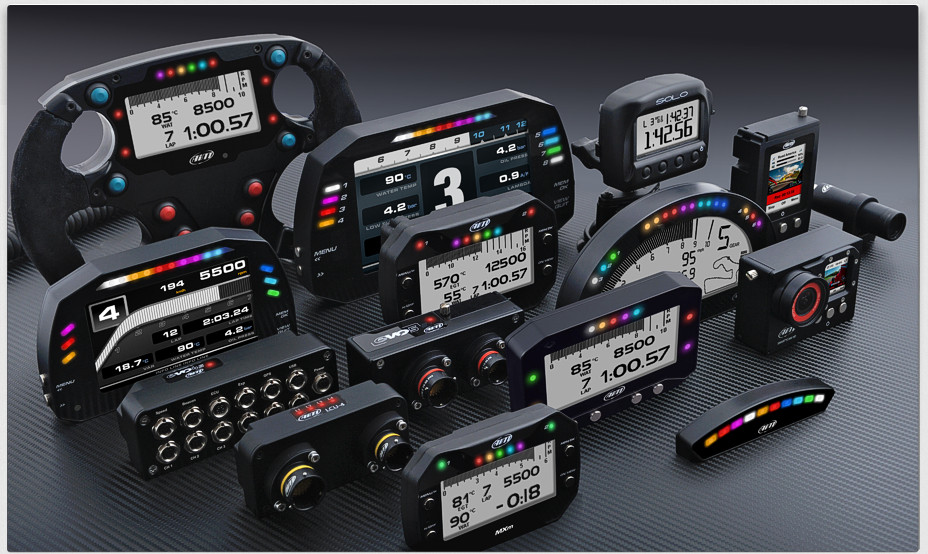
\includegraphics[width=\textwidth]{../common/images/aim-products.jpg}

    \column{0.5\textwidth}
    \begin{itemize}
    \item Embedded Linux engineer\\
      at AIM Sportline\\
      {\footnotesize\href{http://www.aim-sportline.com/}{www.aim-sportline.com}}
      \begin{itemize}
      \item Develop products on custom hardware
      \item Kernel, drivers, bootloader, FPGA
      \item Integration, build system
      \end{itemize}
    \item Open source enthusiast
      \begin{itemize}
      \item Contributor to the Linux kernel, U-Boot, Buildroot and others
      \end{itemize}
    \end{itemize}
  \end{columns}
\end{frame}


\begin{frame}{Contents}
  \tableofcontents
\end{frame}


\section{Video serdes chips}

\begin{frame}{Serializer/deserializers chipset}
  \center\includegraphics[height=0.30\textheight]{images/sensor-soc.pdf}
  \pause
  \center\includegraphics[height=0.30\textheight]{images/sensor-ser-des-soc.pdf}
\end{frame}

\begin{frame}{Typical application}
  \begin{itemize}
  \item Typical use: automotive
    \begin{itemize}
    \item Autonomous driving (ADAS) cameras
    \item Rear camera
    \item Infotainment display
    \end{itemize}
  \item SoC-centric
  \item Cameras/displays model well known in advance
  \item Cameras/displays always connected
  \item High electrical noise
  \end{itemize}
\end{frame}

\begin{frame}{My application}
  \begin{itemize}
  \item Action camera
  \item Base module (SoC, processing, storage)
  \item Two {\em hot-plug} camera modules
    \begin{itemize}
    \item Interchangeable
    \item While recording from the other module
    \item Possibly with a different model
    \end{itemize}
  \end{itemize}
\end{frame}

\begin{frame}{Available serdes chips}
  \begin{itemize}
  \item Main competitors
    \begin{itemize}
    \item Texas Instruments
      \myhref{http://www.ti.com/interface/fpd-link-serdes/products.html}{FPD-Link}
    \item Maxim
      \myhref{https://www.maximintegrated.com/en/products/interface/high-speed-signaling/gmsl-serdes.html}{GMSL}
    \end{itemize}
  \item Camera or display
  \item Video bus: MIPI CSI-2, Sub-LVDS, parallel
  \item Robust link in high electrical noise environment
  \item 1 to 4 inputs per serializer
  \item Most have remote I2C, GPIO
  \item Some have remote UART, audio
  \end{itemize}
\end{frame}

\begin{frame}{Texas Instruments DS90UB954 and DS90UB953}
  \center\includegraphics[height=0.80\textheight]{images/ti-2-cameras.pdf}
\end{frame}


\section{Linux support}

\begin{frame}{Existing patches}
  \myhref{https://lore.kernel.org/linux-media/20181102154723.23662-1-kieran.bingham@ideasonboard.com/}
         {\tt [PATCH v4 0/4] MAX9286 GMSL Support}
  \begin{itemize}
  \item By Kieran Bingham, Laurent Pinchart, Jacopo Mondi, Niklas Söderlund
  \item For Maxim GMSL chips
  \item See also the
    \myhref{https://www.slideshare.net/KieranBingham/gmsl-in-linux}
           {ALS 2018 talk slides}
  \end{itemize}

  \pause
  \myhref{https://lore.kernel.org/linux-media/20181008211205.2900-1-vz@mleia.com/}
         {\tt [PATCH 0/7] mfd/pinctrl: add initial support of TI DS90Ux9xx ICs}
  \begin{itemize}
  \item By Vladimir Zapolskiy
  \item For TI DS90Ux9xx chips
  \item See also the
    \myhref{https://schd.ws/hosted_files/ossalsjp18/8a/vzapolskiy_als2018.pdf}
           {ALS 2018 talk slides}
  \end{itemize}

  \pause
  \myhref{https://lore.kernel.org/linux-media/20190723203723.11730-1-luca@lucaceresoli.net/}
         {\tt [RFC,v2 0/6] TI camera serdes and I2C address translation}
  \begin{itemize}
  \item By Luca Ceresoli
  \item For TI DS90Ux9xx chips
  \item See also: this talk :)
  \end{itemize}
\end{frame}

\begin{frame}{Ideal implementation}
  \center\includegraphics[height=0.80\textheight]{images/implementation-ideal.pdf}
\end{frame}

\begin{frame}{Ideal implementation}
  \begin{itemize}
  \item Similar to BBB capes, RPi hats, but hot-plug
  \item I2C EEPROM on each camera (fixed slave address)
  \item When a camera is connected
    \begin{enumerate}
    \item Add serializer, I2C adapter, GPIO chip
    \item Add I2C EEPROM, read model ID
    \item Insert model-specific device tree overlay
    \item DTO adds sensor and other remote devices
    \end{enumerate}
  \item On disconnection, remove overlay
  \end{itemize}
\end{frame}


\section{Troubles and tribulations}

\begin{frame}{V4L2 troubles}
  \begin{columns}
    \column{0.7\textwidth}
    \begin{flushright}
      The ideal pipeline \textrightarrow
    \end{flushright}

    \vspace{0.2\textheight}

    \begin{enumerate}
    \item Stream multiplexing: no support in mainline yet
    \item Reliability: pipe should work with some nodes disabled
      \begin{itemize}
      \item A sensor goes faulty
      \end{itemize}
    \item Dynamic pipe: remove some nodes, add different ones
      \begin{itemize}
      \item A sensor is removed, a different model added
      \end{itemize}
    \end{enumerate}

    \column{0.3\textwidth}
    \center\includegraphics[height=0.95\textheight]{images/v4l2-ideal-pipe.pdf}
  \end{columns}
\end{frame}

\begin{frame}[fragile]{Devicetree troubles}
  \begin{columns}
    \column{0.7\textwidth}
    \begin{enumerate}
    \item Runtime DT insertion/removal not in mainline yet
    \item Video pipelines: bidirectional endpoints links
    \end{enumerate}

    \begin{minted}[frame=single,autogobble,fontsize=\small]{text}
        deser@30 {                               // base DT
          ports {
            port@0 {
              deser_input: endpoint {
                remote-endpoint = <&ser_output>;
    \end{minted}

    \begin{minted}[frame=single,autogobble,fontsize=\small]{text}
        ser@3d {                              // DT overlay
          ports {
            port@1 {
              ser_output: endpoint {
                remote-endpoint = <&deser_input>;
    \end{minted}

    \column{0.3\textwidth}
    \center\includegraphics[height=0.95\textheight]{images/v4l2-ideal-pipe.pdf}
  \end{columns}
\end{frame}


\section{Way out}

\begin{frame}{Work around main blockers}
  \begin{itemize}
  \item Main blockers for hotplug applications
    \begin{itemize}
    \item Non-modifiable pipeline
    \item Runtime Device Tree overlays
    \end{itemize}
    \pause
  \item Workaround: sensors always instantiated
    \begin{itemize}
    \item V4L2 is happy
    \item Device Tree is static
    \item Sensor driver becomes a hack
    \end{itemize}
    \pause
  \item Goal: segregate workarounds, keep serdes drivers clean
  \end{itemize}
\end{frame}

\begin{frame}{I2C: ideal solution}
  \center\includegraphics[width=0.80\textwidth]{images/i2c-ideal.pdf}
\end{frame}

\begin{frame}{I2C: proposed solution}
  \center\includegraphics[width=0.80\textwidth]{images/i2c-real.pdf}
\end{frame}

\begin{frame}{Remote GPIO}
  \center\includegraphics[height=0.85\textheight]{images/gpio-routing.pdf}
\end{frame}

\begin{frame}{Remote GPIO}
  \center\includegraphics[width=0.80\textwidth]{images/gpio-real.pdf}
\end{frame}


\section{Remote I2C}

\begin{frame}{Remote I2C}
  \begin{itemize}
  \item Different between TI and Maxim chips
  \item Discussed in {\tt linux-i2c}
  \item BoF during Linux Plumbers Conference 2019
    \begin{itemize}
    \item \url{https://lucaceresoli.net/plumbers-i2c-bof}
    \item \url{https://etherpad.openstack.org/p/2019-09-11-I2C-BoF}
    \end{itemize}
  \end{itemize}
\end{frame}

\begin{frame}{Maxim GMSL: I2C switch}
  \begin{center}
    \includegraphics[width=0.90\textwidth]{images/i2c-maxim.pdf}
  \end{center}

  \begin{itemize}
  \item SER+DES are equivalent to an I2C switch
  \end{itemize}
\end{frame}

\begin{frame}{TI FPD-Link III: Address Translation (ATR)}
  \begin{center}
    \includegraphics[width=0.90\textwidth]{images/i2c-ti.pdf}
  \end{center}

  \begin{itemize}
  \item I2C transactions are replicated based on an alias table
  \end{itemize}
\end{frame}

\begin{frame}[fragile]{Address Translation (ATR)}
  \begin{Verbatim}[commandchars=\\\{\}]
# i2cdetect -l
i2c-0    i2c           amba:camera-i2c@0                   I2C adapter
i2c-4    i2c           i2c-0-atr-0                         I2C adapter
i2c-5    i2c           i2c-0-atr-1                         I2C adapter
# \pause{}echo eeprom \textcolor{red}{0x0a} > /sys/bus/i2c/devices/\textcolor{blue}{i2c-4}/new_device
# \pause{}dmesg | tail -n2
ds90ub954 0-0030: rx0: client \textcolor{red}{0x0a} mapped at alias \textcolor{green}{0x4b} (eeprom)
i2c \textcolor{blue}{i2c-4}: new_device: Instantiated device eeprom at \textcolor{red}{0x0a}
# \pause{}hexdump /sys/bus/i2c/devices/\textcolor{blue}{4}-\textcolor{red}{000a}/eeprom
0000000 ffff ffff ffff ffff ffff ffff ffff ffff
*
0000100
#
  \end{Verbatim}
\end{frame}


\section{Conclusions}

\begin{frame}{Conclusions}
  \begin{itemize}
  \item Video serdes are complex
  \item Issues for proper implementation
    \begin{itemize}
    \item V4L2 limitations
    \item Additional limitations for hotplug (V4L2, Device Tree overlays)
    \item There's a workaround, implies some compromise
    \end{itemize}
  \item There is a plan for proper implementation of remote I2C (on TI chips)
  \end{itemize}
\end{frame}

\begin{frame}
  \begin{columns}
    \column{0.4\textwidth}
    \center

    {\Huge Questions?}

    \column{0.6\textwidth}
    \center

    {\Large Thank you for your attention!}

    \vspace{0.15\textheight}

    {\Large Luca Ceresoli}\\
    \href{mailto:luca@lucaceresoli.net}{luca@lucaceresoli.net}\\
    \url{http://lucaceresoli.net}

    \vspace{0.05\textheight}

    \tiny
    \textcopyright{} Copyright 2019, Luca Ceresoli\\
    Slides released under\\
    Creative Commons Attribution - Share Alike 3.0 License \\
    \url{https://creativecommons.org/licenses/by-sa/3.0/} \\
\end{columns}
\end{frame}

\end{document}
